%!TEX root = main.tex
\section{Описание предприятия}

Следственный комитет Российской Федерации --- федеральный государственный орган в России, осуществляющий полномочия в сфере уголовного судопроизводства. Является государственной военизированной организацией. Наделен правом ведения предварительного следствия и дознания.

Экспертно-криминалистический отдел является структурным подразделением Следственного управления следственного комитета России по Иркутской области и производит судебные экспертизы (исследования) в соответствии с требованиями и положениями действующего законодательства и экспертных методик.

СК~РФ образован на базе Следственного комитета при прокуратуре Российской Федерации\cite{order33}. Начал свою деятельность 15~января~2011 года. Началом деятельности экспертно-криминалистического отдела является 20~октября~2014~г.\cite{order71}

\subsection{Организационная структура предприятия}

Следственный комитет России находится в непосредственном подчинении Президента~РФ. Руководитель --- Бастрыкин Александр Иванович. Главой Следственного управления СК РФ по Иркутской области является Бунёв Андрей Юрьевич.

Экспертно-криминалистический отдел возглавляет Себякин Алексей Геннадьевич.

\begin{figure}[H]
	\centering
	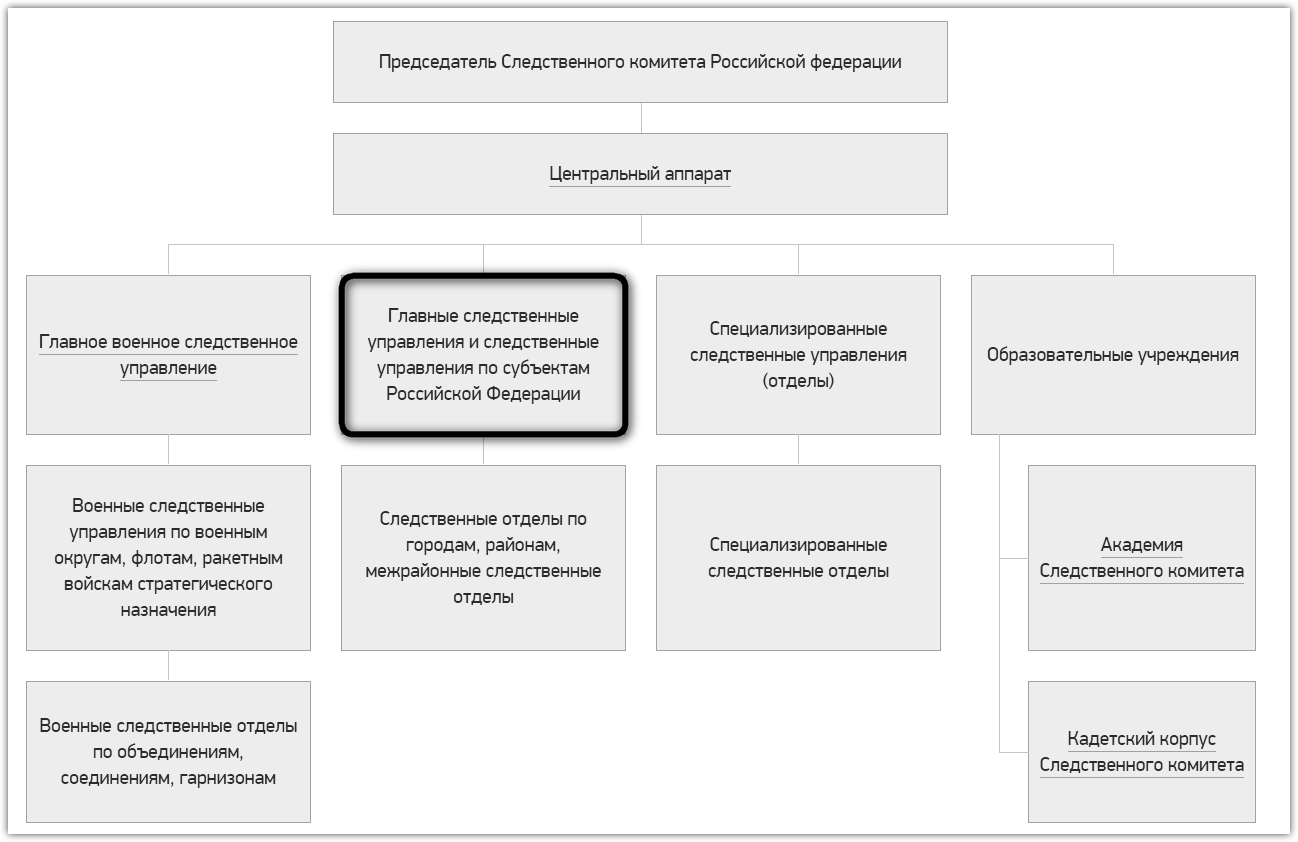
\includegraphics[width=0.8\textwidth]{pics/general_struct.png}
	\caption{Организационная структура Следственного комитета РФ}
	\label{fig:org_struct}
\end{figure}

На рисунке~\ref{fig:org_struct} выделена группа подразделений, к которой относится Следственное управление Следственного комитета РФ по Иркутской области (частью которого является экспертно-криминалистический отдел), которое состоит из следующих отделов~\cite{sled:struct}:

\begin{itemize*}
	\item организационно-контрольный отдел;
	\item отдел кадров;
	\item отдел процессуального контроля;
	\item отдел обеспечения собственной безопасности и физической защиты;
	\item отдел криминалистики;
	\item экспертно-криминалистический отдел;
	\item отдел материально-технического обеспечения;
	\item финансово-экономический отдел;
	\item отдел по приему граждан и документационному обеспечению;
	\item первый отдел по расследованию особо важных дел;
	\item второй отдел по расследованию особо важных дел;
	\item третий отдел по расследованию особо важных дел.
\end{itemize*}

В состав отдела входят 1 заместитель, 3 старших эксперта, 5 экспертов. Распределение специализаций между старшими экспертами и экспертами отдела и их взаимозаменяемость осуществляются в соответствии с распоряжением руководителя Следственного управления №29-246р.\cite{29-246}

\begin{figure}[H]
	\centering
	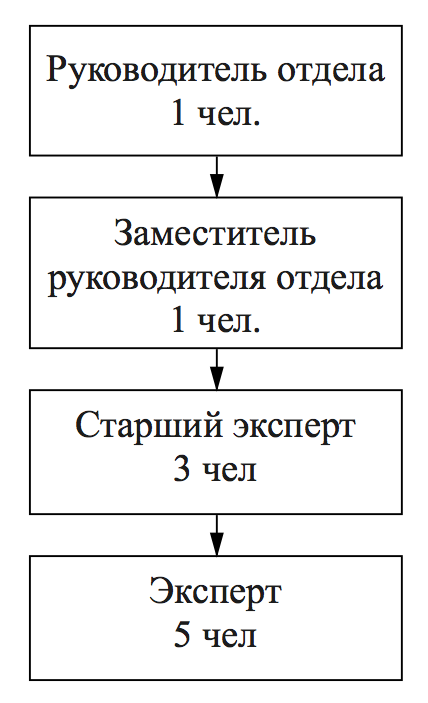
\includegraphics[width=0.3\textwidth]{pics/func_struct.png}
	\caption{Функциональная структура экспертно-криминалистического отдела Следственного управления Следственного комитета РФ по Иркутской области}
\end{figure}

\subsection{Основные направления деятельности}

Экспертно-криминалистический отдел Следственного управления Следственного комитета РФ по Иркутской области занимается широким спектром исследований. Главными можно выделить следующие виды экспертиз:

\begin{enumerate*}
	\item компьютерно-техническая;
	\item информационно-аналитическая;
	\item видеотехническая;
	\item лингвистическая;
	\item фоноскопическая;
	\item экономическая;
	\item психофизиологическая экспертиза с использованием полиграфа;
	\item иные экспертизы, в соответствии с организационно-распорядительными документами СК России и Следственного управления.
\end{enumerate*}

\subsection{Функциональные обязанности сотрудников отдела}

За каждым сотрудником экспертно-криминалистического отдела закреплена одна или несколько обязанностей, из представленных ниже:

\begin{enumerate*}
\item Проведение компьютерно-технических экспертиз и исследований. При производстве экспертиз и исследований решаются следующие задачи:
	\begin{itemize*}
		\item диагностика аппаратных средств и их составных частей в целях установления их технического состояния;
		\item исследование носителей с целью поиска заданной информации;
		\item поиск латентной и закодированной информации на носителях информации;
		\item исследование фрагментов информации в целях ее реконструкции;
		\item исследование компьютерных систем для установления возможности решения конкретных преступных задач;
		\item исследование программ для ЭВМ и баз данных для определения их предназначения, работоспособности и потребительских свойств.
	\end{itemize*}
	\item Проведение информационно-аналитических экспертиз и исследований. При производстве экспертиз и исследований решаются следующие задачи:
	\begin{itemize*}
		\item анализ детализаций телефонных соединений абонентских номеров;
		\item анализ массивов данных систем распознавания государственных регистрационных знаков автотранспортных средств;
		\item анализ массивов данных систем обслуживания магнитных пластиковых карт.
	\end{itemize*}
	\item Проведение	видео-технических	экспертиз	и	исследований.	При
производстве экспертиз и исследований решаются следующие задачи:
	\begin{itemize*}
		\item улучшениеие качества видеозаписи;
		\item идентификация средств видеозаписи;
		\item установление признаков внесения изменений в видеозапись.
	\end{itemize*}
	\item Проведение	лингвистических	экспертиз	и	исследований.	При
производстве экспертиз и исследований решаются следующие задачи:
	\begin{itemize*}
		\item семантический анализ текстов;
		\item лингвистический анализ продуктов речевой деятельности.
	\end{itemize*}
	\item Проведение	фоноскопических	экспертиз	и	исследований.	При
производстве экспертиз и исследований решаются следующие задачи:
	\begin{itemize*}
		\item идентификация личности по голосу и устной речи;
		\item идентификация средств звукозаписи, идентификация источников звуков;
		\item установление дословного содержания разговора;
		\item определение количества участников разговора;
		\item установление признаков внесения изменений в аудиозапись.
	\end{itemize*}
	\item Проведение экономических экспертиз и исследований. При производстве экспертиз и исследований решаются следующие задачи:
	\begin{itemize*}
		\item исследование отражения в первичных учетных, иных первичных документах, регистрах учета (бухгалтерского и налогового), отчетности (бухгалтерской и налоговой) фактов финансово-хозяйственной деятельности, имущества и обязательств исследуемого лица;
		\item исследование соответствия порядка отражения фактов финансовохозяйственной деятельности, имущества и обязательств в первичных учетных, иных первичных документах, регистрах учета (бухгалтерского и налогового), отчетности (бухгалтерской и налоговой), реализованного хозяйствующим субъектом, правилам бухгалтерского и надогового учета;
		\item исследование финансового состояния хозяйствующего субъекта;
		\item исследование соблюдения принципов кредитования.
	\end{itemize*}
	\item Проведение психофизиологических экспертиз и исследований. Целью проведения психофизиологических экспертиз и исследований является проверка достоверности информации, сообщаемой обследуемым лицом, при решении задач:
	\begin{itemize*}
		\item уголовного судопроизводства;
		\item отбора кадров при приеме граждан на службу (работу) в СК России;
		\item служебной деятельности при проведении служебных проверок в системе СК России.
	\end{itemize*}
\end{enumerate*}


\subsection{Основные задачи}
К задачам отдела относятся:
\begin{itemize*}
	\item производство судебных экспертиз и экспертных исследований в соответствии с постановлениями и поручениями должностных лиц Следственного управления, наделенных правом назначения судебных экспертиз в соответствии с действующим законодательством Российской Федерации;
	\item проведение научно-исследовательских работ по теоретическим и методическим проблемам в области судебной экспертизы;
	\item создание и совершенствование методик экспертного исследования, а также внедрение новых методов и методик в судебно-экспертную практику;
	\item осуществление работы, направленной на повышение квалификации и подготовку экспертных кадров;
	\item оказание методической помощи сотрудникам правоохранительных органов и судам по вопросам назначения и производства судебных экспертиз и экспертных исследований, проводимых в ЭКО;
	\item производство судебных экспертиз и экспертных исследований по заданиям должностных лиц правоохранительных органов и судов в случаях подбора необходимых материалов для проведения обобщения экспертной практики, научно- исследовательской и методической работы.
\end{itemize*}

\subsection{Алгоритм проведения экспертиз}

Все вещественные доказательства (системные блоки, жесткие диски, другие носители информации), направленные на экспертизу, подлежат описи и сопровождаются приказом, в котором указываются:

\begin{itemize*}
	\item информация об уголовном деле, в котором фигурируют данные вещественные доказательства;
	\item перечень необходимых экспертиз;
	\item перечень вопросов, которые необходимо раскрыть в отчете.
\end{itemize*}

Алгоритм проведения стандартной экспертизы имеет вид, представленный на рисунке~\ref{fig:research_order}

\begin{figure}[H]
	\centering
	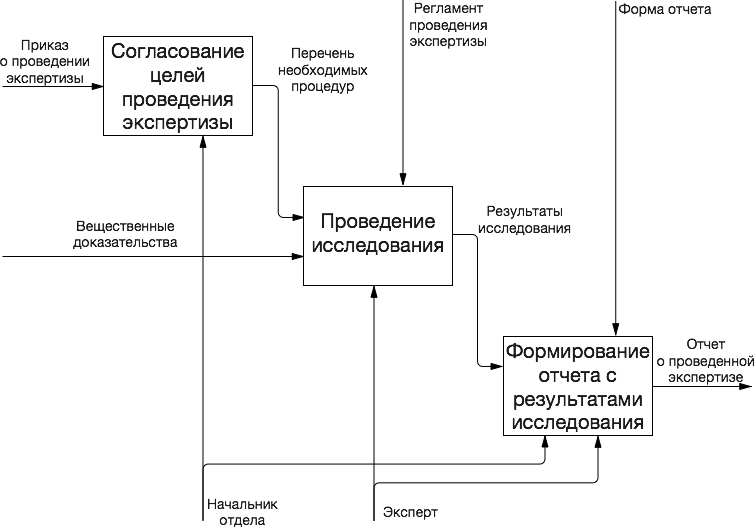
\includegraphics[width=0.8\textwidth]{pics/research_order.png}
	\caption{Организационная структура Следственного комитета РФ}
	\label{fig:research_order}
\end{figure}

